\newcommand{\texMacro}[2]{\texttt{\textbackslash{#1}\{#2\}}}
\section{Part 5.2 Identification of the wave spectrum model}
\subsection{A, Estimating the Power Spectral Density function of $\psi_w$}
In this part we wish to estimate the Power Spectral Density- (PSD) function of how the waves impact the heading.  
Given data of how the waves influence the compass measurement, $\psi_w$ , we can find the PSD-function, named $S_{\psi_w}(\omega)$, using MATLAB. In \cref{PSD func matlab} we show how we calculated the PSD-function.\\
psi\_w is a data series of $\psi_w$, given in degrees. We scale it to radians.  
\begin{lstlisting}[caption={Calculating Power Spectral Density function},label={PSD func matlab}]
x = psi_w(2,:)*pi/180;
fs = 10;
[pxx,f] = pwelch(x,window, [], [], fs);
pxx=pxx./(2*pi);
f=f.*2*pi;
\end{lstlisting} 
Plotting (pxx, f), which is  $S_{\psi_w}$, we get \Cref{fig:Power Spectral density}. 
\begin{figure}
    \centering
    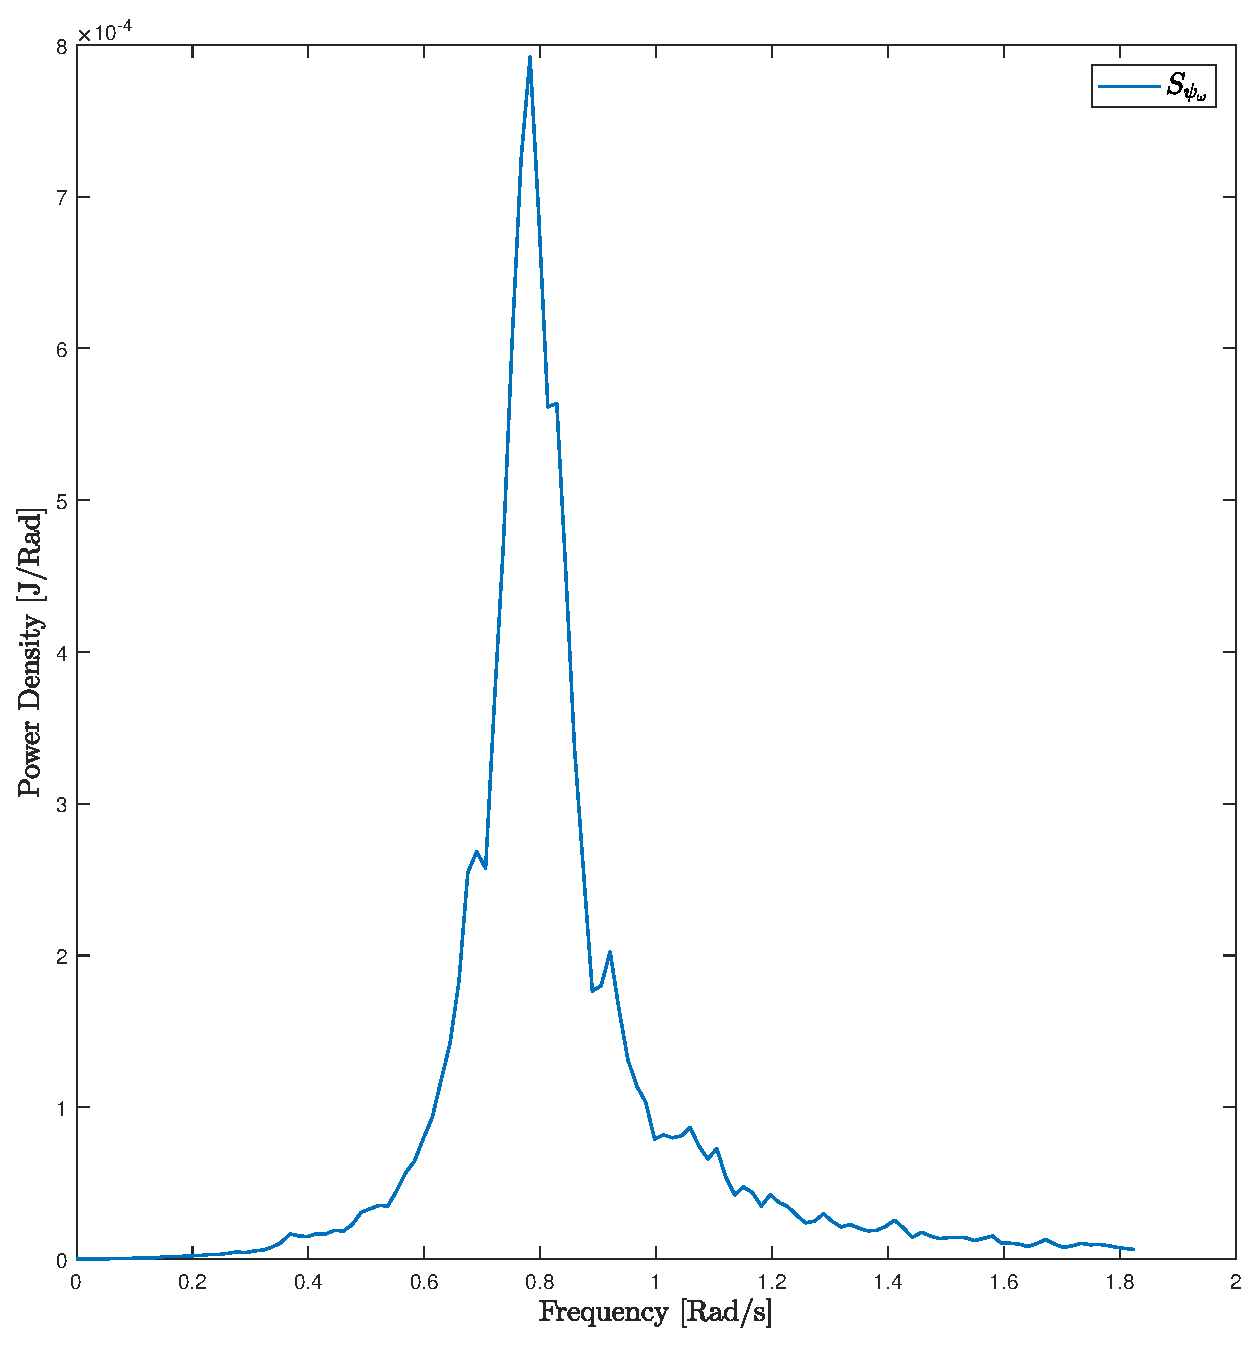
\includegraphics[width=1.00\textwidth]{figures/plots/P5p2a_PSD.eps}
    \caption{Power Spectral Density function for compass measurement}
    \label{fig:Power Spectral density}
\end{figure}


\subsection{B, Analytical expression for the Power Spectral Density}
Analytical expression for the transfer function of the wave response model

From \cite{assignment} we have the Namoto equations
\begin{align}
    \dot{\xi}_w &= \psi_w\label{eq:namoto1}\\
    \dot{\psi}_w &= -\omega_0^2\xi_w-w\lamda\omega_0\psi_w+K_{w}w_w\label{eq:namoto2}
\end{align}
Taking the Laplace transform of these and inserting \ref{eq:namoto1} into \ref{eq:namoto2} we get
\begin{align*}
    s\xi_w &= \psi_w\\
    s\psi_w &= -\omega_0^2\frac{\psi}{s} - w\lamda\omega_0\psi_w + K_{w}w_w\\
    (s^2+2\lambda\omega_0+\omega_0^2)\psi_w &= K_{w}w_w\\
    \frac{\psi_w}{w_w}(s) &= \frac{K_{w}s}{s^2+2\lamda\omega_0s+\omega_0^2}\\
    \hat{H}(j\omega) &= \frac{K_{w}s}{s^2+2\lamda\omega_0s+\omega_0^2}
\end{align*}
where $\hat{H}(j\omega)$ is the transfer function from $w_w$ to $\psi_w$.

Using the Wiener-Khinchin theorem \cite{Wiener-Kinchkin} we can find an analytical expression for the Power Spectral Density function for $\psi_w$. 
Using that $w_w$ is a zero mean white noise, we know that the Power Spectral Density function of $w_w$, called $P_{w_{w}}$, is 1. Thus we get that 
\begin{align*}
    P_{\psi_{w}} &= P_{w_w}\abs{\hat{H}(j\omega)}^2\\
    &= \hat{H}(-j\omega)\hat{H}(j\omega)\\
    &= \hat{H}(-j\omega)\hat{H}(j\omega)\\
    &= \hat{H}(-j\omega)\hat{H}(j\omega)\\
    &= \frac{(K_{w}j\omega)(-K_{w}j\omega)}{((j\omega)^2+2\lamda\omega_0j\omega+\omega_0^2)(-j\omega)^2-2\lamda\omega_0j\omega+\omega_0^2)}\\
    &= \frac{K_{w}^2\omega^2}{\omega^4+\omega^2\omega_0^2(4\lambda^2-2)+\omega_0^4}
\end{align*}


\subsection{C, Finding $\omega_0$ and $\sigma^2$}
Reading the values from \cref{fig:Power Spectral density} we get
\begin{align*}
    \omega_0 &= 0.07823\\
    \sigma &= 0.0281
\end{align*}
where $\omega_0$ is the frequency of peak intensity, and $\sigma^2$ is the peak frequency. 


\subsection{D, Identifying the dampening factor $\lambda$}
We want to identify the damping factor $\lambda$. Using 
$$K_w = 2\lambda\omega_0\sigma$$ 
we get 
$$P_{\psi_{w}} = \frac{4\lambda^2\omega_0^2\sigma^2\omega^2}{\omega^4+(4\lambda^2-2)\omega_0^2\omega^2+\omega_0^4}$$
By plotting $P_{\psi_w}$ versus $S_{\psi_w}$ and adjusting $\lambda$ until the plots overlay we find an estimate for $\lambda$. 

Thus we found that a decent value for lambda is $\lambda  = 0.09$. This value gave $P_{\psi_w}$ shown in \Cref{fig:PSD P vs S} plotted versus $S_{\psi_w}$.


\begin{figure}
    \centering
    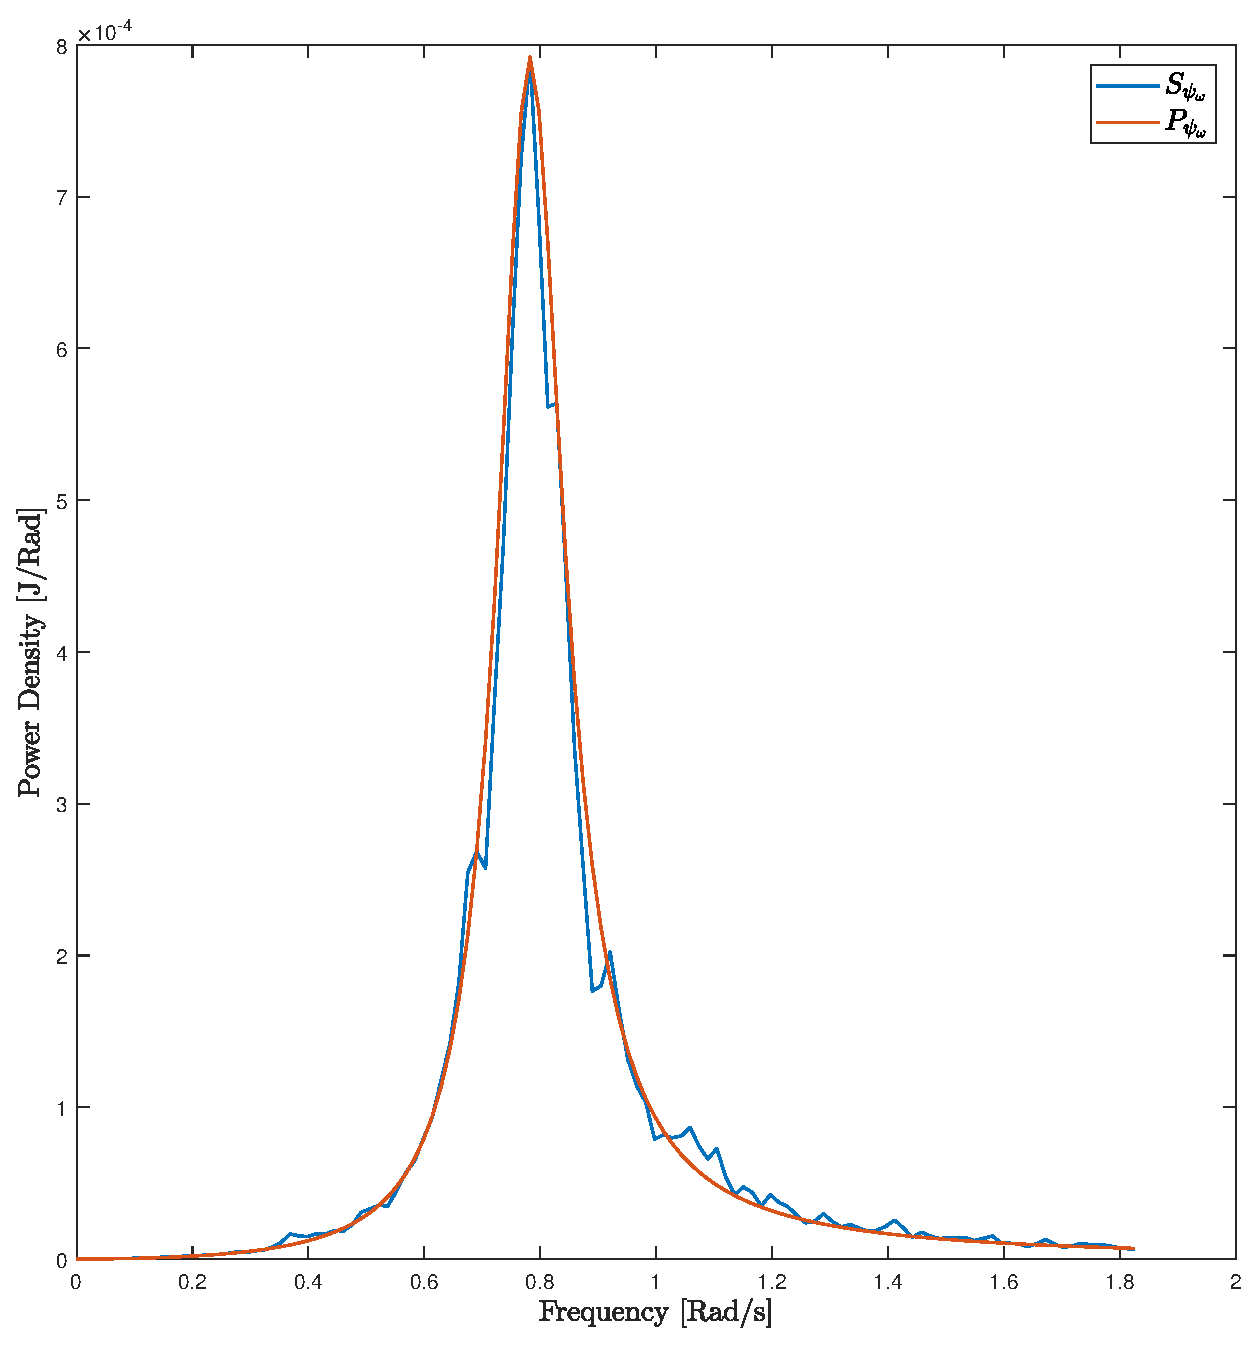
\includegraphics[width=1.00\textwidth]{figures/plots/P5p2d_lambda009rad.eps}
    \caption{$P_{\psi_w}$ plotted versus $S_{\psi_w}$, $\lambda$ = 0.09}
    \label{fig:PSD P vs S}
\end{figure}




